\subsection{Aufbau}
\begin{minipage}{0.5 \linewidth}
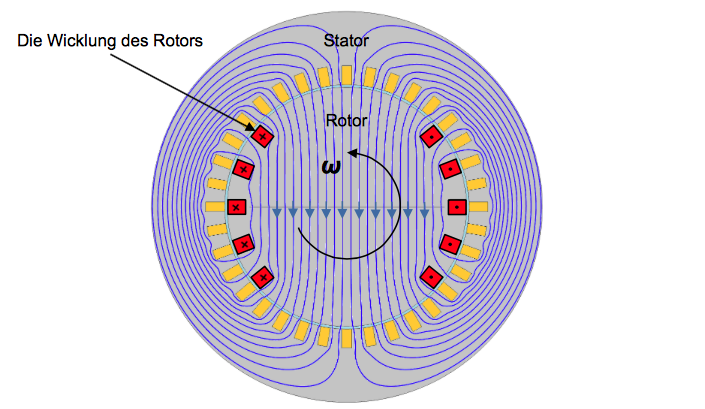
\includegraphics[width = \linewidth]{./Pics/VL1011/Aufbau}
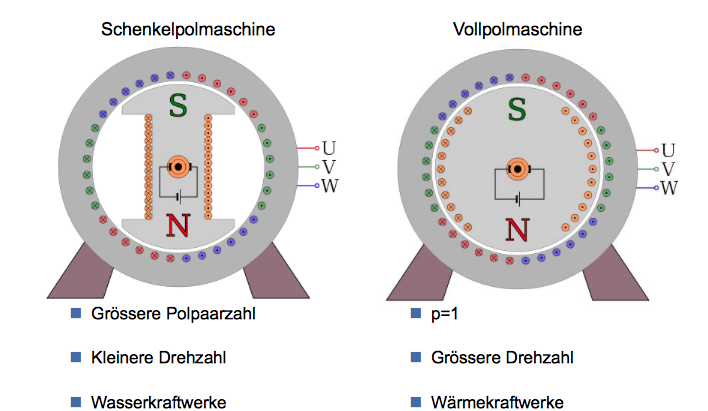
\includegraphics[width = \linewidth]{./Pics/VL1011/Aufbau3}
\end{minipage}
\begin{minipage}{0.5 \linewidth}
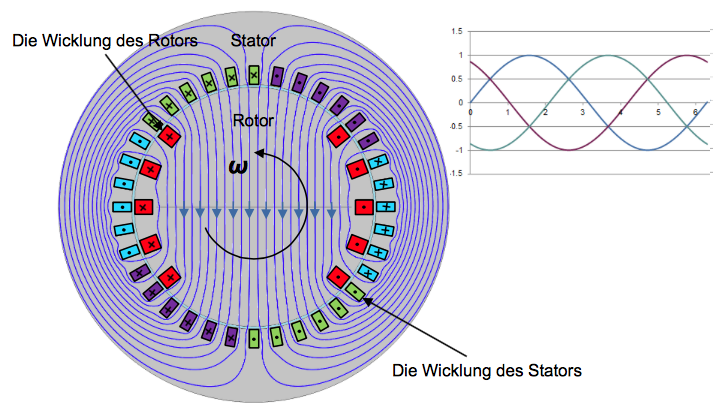
\includegraphics[width = \linewidth]{./Pics/VL1011/Aufbau2}
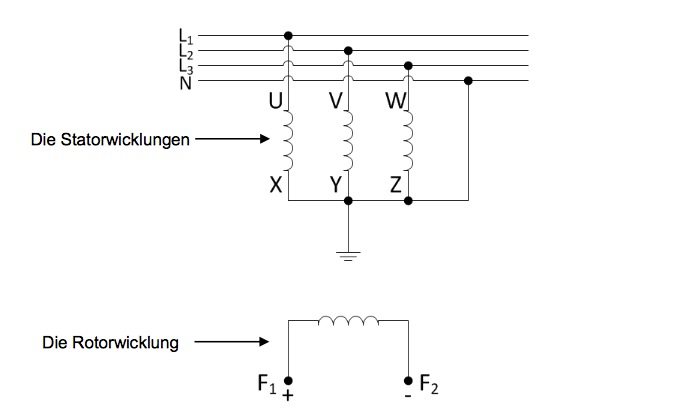
\includegraphics[width = \linewidth]{./Pics/VL1011/Aufbau4}
\end{minipage}

\subsection{Grundgleichungen}
\begin{minipage}{0.4 \linewidth}
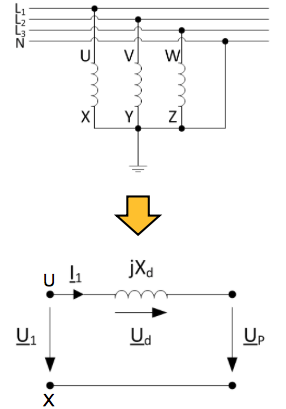
\includegraphics[width = \linewidth]{./Pics/VL1011/Grundgleichung}
\includegraphics[width = \linewidth]{./Pics/VL1011/leerlaufk}
\includegraphics[width = \linewidth]{./Pics/VL1011/kurzschlussk}
\end{minipage}
\begin{minipage}{0.5 \linewidth}
Die Annahme der Analyse: 
\begin{itemize}
\item Die drei Stränge der Synchronmaschine sind gleich ausgelegt.
\item Die Stränge der Maschine haben gleichen Strang-Widerstand $R_s$ und gleiche Strang-Induktivität $L_s$.
\item Die Maschine ist an ein symmetrisches Sinus-Drehstromnetz angeschlossen.
\end{itemize}
Die Vereinfachung der Analyse, die Annahme entspricht:
\begin{itemize}
\item Es braucht nur ein Strang der Maschine in der Analyse betrachtet werden.
\end{itemize}

\begin{itemize}
\item Das magnetische Luftspaltfeld der Maschine, das die Leistung und das Drehmoment der Maschine bestimmt, wird durch die Kopplung des Stator-Drehfelds und Rotor-Magnetfelds modelliert.
\item Der Luftspalt der Maschine wird durch die so genannte Synchronreaktanz der Maschine $X_d$ dargestellt.
\item $\underline{U_1} = \underline{U_d} + \underline{U_p}$
\item $\underline{U_d} = jX_d \cdot \underline{I_1}$
\item $X_d = X_{\sigma 1} + X_h$
\item wobei $U_1$ die Strangspannung, $X_d$ die Synchronreaktanz, $X_{\sigma 1}$ die Streureaktanz des Stators, $X_h$ die Hauptreaktanz und $U_p$ die so genannte Polradspannung ist.
\item Die Polradspannung ist eine fiktive Hilfsgrösse. Im Leerlauf der Maschine entspricht die Polradspannung der von dem Erregerstrom induzierten Spannung der Statorwicklung. 
\item $\underline{U_P} = \underline{U_P}(I_e)$
\item $\underline{U_P} = jX_h \cdot I_e'$
\item wobei $I_e'$ der Erregerstrom umgerechnet auf die Statorseite ist.
\item Gemäss dem präsentierten mathematischen Model lässt sich die Synchronreaktanz von den Ergebnissen des Leerlauf- und Kurzschlussversuchs ermitteln.
\end{itemize}
\end{minipage}

\subsection{Zeigerdiagramm im Generator- und Motorbetrieb}
\begin{minipage}{0.5 \linewidth}
\subsubsection{Motorbetrieb}
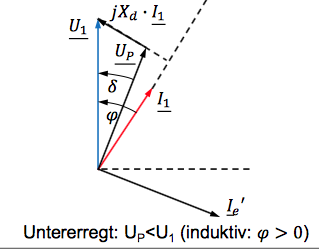
\includegraphics[width = 0.5 \linewidth]{./Pics/VL1011/motuntererregt}
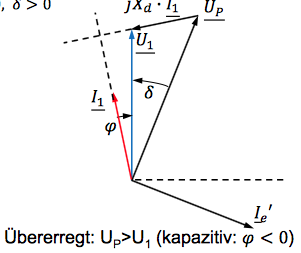
\includegraphics[width = 0.5 \linewidth]{./Pics/VL1011/motuebererregt}
\end{minipage}
\begin{minipage}{0.5 \linewidth}
\subsubsection{Generatorbetrieb}
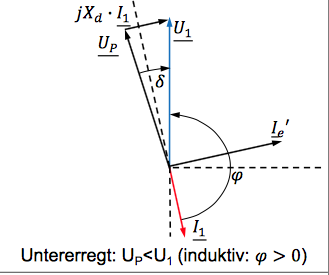
\includegraphics[width = 0.5 \linewidth]{./Pics/VL1011/genuntererregt}
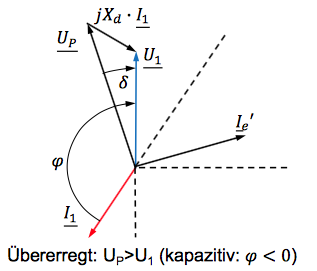
\includegraphics[width = 0.5 \linewidth]{./Pics/VL1011/genuebererregt}
\end{minipage}

\subsection{Leistung}
\begin{minipage}{0.25 \linewidth}
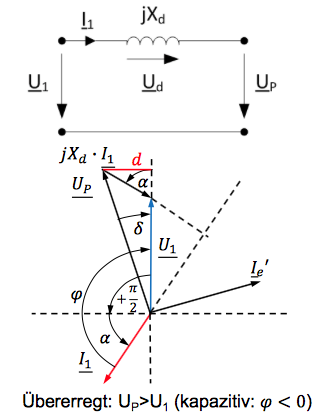
\includegraphics[width =  \linewidth]{./Pics/VL1011/Leistung}\\
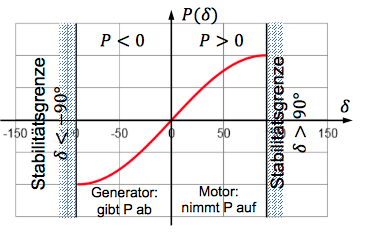
\includegraphics[width =  \linewidth]{./Pics/VL1011/Leistung2}
\end{minipage}
\begin{minipage}{0.5 \linewidth}
Der Polradwinkel: $\delta = \angle(U_p, U_1)$ \\

$\varphi = -\alpha - \frac{\pi}{2}$\\
$cos\varphi = -sin\alpha$\\

Generatorbetrieb: $\delta < 0$ \\

$d = -U_p \cdot sind\delta = X_d\cdot I_1 \cdot sin\alpha = -X_d\cdot I_1\cdot cos\varphi$ \\

$P = 3 \cdot U_1 \cdot I_1 \cdot cos\varphi$\\

$P(\delta) = 3 \frac{U_p\cdot U_1}{X_d} sin\delta$\\

Generator: $P(\delta) = P_{mech} - P_v = \omega \cdot M - P_v$ \\

Motor: $P(\delta) = P_{mech} + P_v = \omega \cdot M + P_v$ \\
\end{minipage}

\subsection{Erreger-Regulierkennlinien}
\begin{minipage}{0.25 \linewidth}
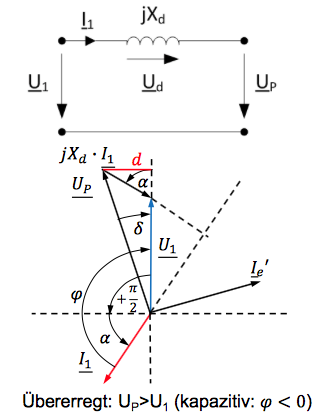
\includegraphics[width =  \linewidth]{./Pics/VL1011/Leistung}
\end{minipage}
\begin{minipage}{0.75 \linewidth}
$U_p^2 = U_1^2 + (X_d I_1)^2 - 2 \cdot U_1 \cdot X_d I_1 \cdot cos(\pi-\alpha)$\\

$cos(\pi - \alpha) = - cos\alpha = sind \varphi$ \\

$U_p^2 = U_1^2 + (X_d I_1)^2 - 2 \cdot U_1 \cdot X_d I_1 \cdot sin\varphi$\\

Die Nennbetriebsidentität: $U_1 = I_N \cdot X_N$ \\

$U_p^2 = (X_N I_N)^2+ (X_d I_1)^2 - 2 \cdot U_1 \cdot X_d I_1 \cdot sin\varphi$\\

$\frac{U_P^2}{U_1^2} = 1 + (\frac{X_d}{X_n} \cdot \frac{I_1}{I_N})^2 - 2 \cdot \frac{X_d}{X_n} \cdot \frac{I_1}{I_N} \cdot sin\varphi$\\

Die Proportionalität: $U_P = k \cdot I_e$ \\

$\frac{I_e^2}{I_{e0}^2} = 1 + (\frac{X_d}{X_n} \cdot \frac{I_1}{I_N})^2 - 2 \cdot \frac{X_d}{X_n} \cdot \frac{I_1}{I_N} \cdot sin\varphi$\\

\end{minipage}

\begin{minipage}{0.25 \linewidth}
\includegraphics[width =  \linewidth]{./Pics/VL1011/regulierkennlinie}
\end{minipage}
\begin{minipage}{0.75 \linewidth}
$\frac{I_e^2}{I_{e0}^2} = 1 + (\frac{X_d}{X_n} \cdot \frac{I_1}{I_N})^2 - 2 \cdot \frac{X_d}{X_n} \cdot \frac{I_1}{I_N} \cdot sin\varphi$\\

$\Rightarrow (\frac{I_e}{I_{e0}})^2 = 1 + (x \cdot \frac{I_1}{I_N})^2 - 2 \cdot x \cdot \frac{I_1}{I_N} \cdot sin\varphi$ \\

Der Bezugswert: $x=\frac{X_d}{X_n}$ \\

$\Rightarrow (\frac{I_e}{I_{e0}})^2 = 1 + (x \cdot \frac{I_1}{I_N} - sin\varphi)^2 - sin^2\varphi$ \\

$\Rightarrow (\frac{I_e}{I_{e0}})^2 = \sqrt{cos^2\varphi + (x \cdot \frac{I_1}{I_N} - sin\varphi)^2}$ \\

Mit der letzten Gleichung sind die so genannten Erreger-Regulierkennlinien $I_e = f(I_1)$ angegeben. \\

Diese Gleichung beantwortet die folgenden Fragen: \\
Welcher Erregerstrom $I_e$ für einen gewünschten Netzstrom $I_1$ bei der Nennspannung $U_N$ eingestellt werden soll, wenn der Induktive oder kapazitive Leistungsfaktor $cos \varphi$ vorgegeben ist. 
\end{minipage}

\subsection{Anwendung}
\begin{itemize}
\item Synchronmaschinen werden hauptsächlich als Drehstromgeneratoren in Kraftwerken verwendet.
\item In Wärmekraftwerken werden Vollpolmaschinen mit der Leistung bis 2000 MVA und mit der Spannung bis 27 kV eingesetzt.
\item In Wasserkraftwerken werden Schenkpolmaschinen mit der Leistung 1000 MVA und mit der Spannung bis 25 kV eingesetzt.
\item Drehstromsynchronmotoren grosser Leistung werden als Antrieb für Gebläse, Pumpe, Verdichter und Bahnantriebe verwendet.
\item Die Drehzahlregulierung der Synchronmotoren wirrd hauptsächlich mit einem Frequenzumrichter durchgeführt.
\end{itemize}